\chapter{Pruebas Ejecutadas} \label{cap:ocho}
Uno de los objetivos presentes en la entrega del trabajo terminal es obtener un producto de calidad y gran valor para el usuario final; para lograr este objetivo es necesario comprobar que cada segmento de la plataforma funcione de la manera esperada y que aporte valor al proceso de creación del documento. Por tal motivo se llevó a cabo la validación y verificación de cada sprint del sistema en la ejecucución de pruebas dinámicas correspondientes, de igual manera y con ayuda de la herramienta SonarQube el producto se sometió a pruebas de código en la ejecución de pruebas estáticas.

\section{Pruebas Dinámicas}

Con base en los enunciados de la ISTQB, se determinó que el nivel de prueba que se requiere para el trabajo terminal se concentra en las pruebas de sistema ya que el tiempo para ejecutar las pruebas es limitado en comparación con el tiempo de desarrollo y análisis; la ventaja de realizar las pruebas en este nivel es que se probará el funcionamiento del sistema completo así como la comunicación dentro de sus módulos.\\

El diseño de pruebas dinámicas está basado en la espeficicación técnica del sistema, la razón principal por la cual se aplicó esta técnica tiene que ver con el sustento documental con el que se cuenta.\\

\subsection{Diseño de Pruebas Dinámicas}

A continuación se detalla el diseño de las pruebas dinámicas basadas en la especificación técnica, así como de las herramientas creadas con base en el análisis de: Clases de equivalencia, Valores frontera, Reglas de negocio, Máquinas de estado y Casos de uso.

\subsubsection{MATRICES DE PRUEBA}

Las matrices son una herramienta que detalla el resultado de la ejecución de pruebas en comparación con cada una de las características y funcionalidades de los módulos del sistema. Están basadas en el documento de análisis, especifícamente en el documento de casos de uso.\\

El objetivo del diseño de estas matrices de prueba es validar y verificar a través de ciclos de pruebas que el producto cumpla con lo espeficicado en las etapas precedentes, en caso de que no se cumpla con las funcionalidades estipuladas o existan mejoras en su implementación se reporta una serie de defectos y sugerencias para que desarrollo se encargue de corregirlos; una vez que se solucionaron los problemas se ejecuta un ciclo de confirmación para comprobar que efectivamente se han corregido los defectos y que no se ha alterado ningúna otra parte del sistema.\\

En la Figura \ref{fig:estructurap} se ilustra la estructura de las matrices de prueba que se diseñaron para registrar el resultado de su ejecución en los ciclos correspondientes.

\begin{figure}[H]
	\begin{center}
		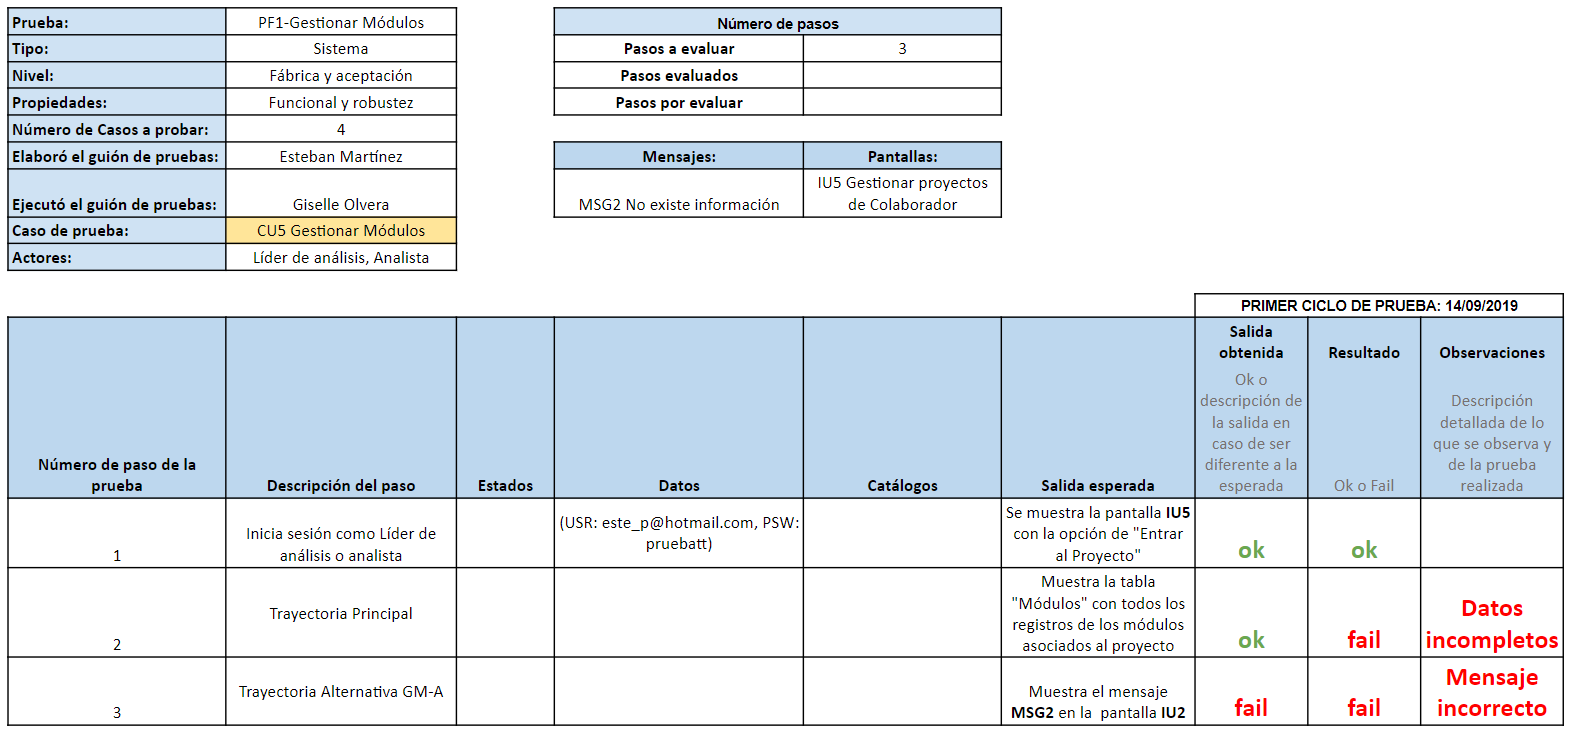
\includegraphics[width=.99\textwidth]{images/pruebas/diseno/estructurap}
		\caption{Ejemplo de la estructura diseñada para la matriz de pruebas}
		\label{fig:estructurap}
	\end{center}
\end{figure}

En la Figura \ref{fig:encabezado} se ilustra la estructura de las matrices de prueba que se diseñaron para registrar el resultado de su ejecución en los ciclos correspondientes.

\begin{figure}[H]
	\begin{center}
		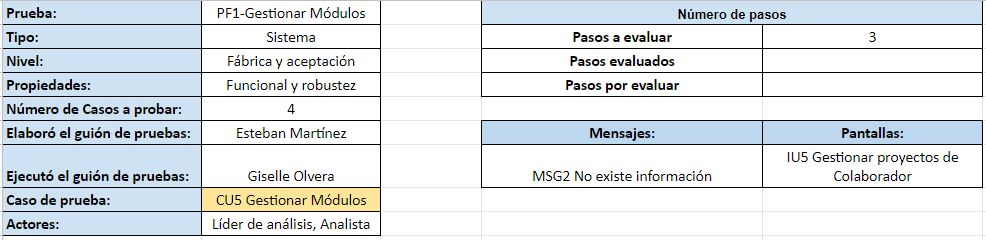
\includegraphics[width=.95\textwidth]{images/pruebas/diseno/encabezado}
		\caption{Ejemplo del encabezado de la matriz de pruebas}
		\label{fig:encabezado}
	\end{center}
\end{figure}

Se implementaron las 5 técnicas para pruebas basadas en espicificación tal y como se enuncia en el ISTQB:

\begin{itemize}
	\item \textbf {Clases de equivalencia}:
	Las clases de equivalencia son particiones que se aplican principalmente en las entradas de datos a través de formulario. Para cada campo se hace una partición con las posibles condiciones que se deberían o no de cumplir de tal manera que para cada prueba solo se ejecute una de las condiciones de dicha partición.
	
	\item \textbf {Valores frontera}:
	Se utilizó como parte de una condición en la clase de equivalencia para verificar que se están cumpliendo los rangos especificados en el diccionario de datos. 
	
	\item \textbf {Reglas de negocio}:
	Al igual que los valores frontera, las reglas de negocio son condiciones que forman parte de las clases de equivalencia, en este caso nos ayudan a definir cuales condiciones se deben cumplir con respecto al negocio. 
	
	\item \textbf {Máquinas de estado}:
	Describimos el comportamiento requerido por la máquina de estados presente en el sistema indicando las acciones habilitadas al encontrarse en un estado en específico.
	
	\item \textbf {Casos de uso}:
	Los casos de uso son la base de prueba más importante que se consideró en el diseño de las matrices, gracias a las trayectorias ya definidas por análisis es posible ejecutar las pruebas de funcionalidad con base en su especificación. Gracias a esta técnica es posible verificar el funcionamiento de un caso de uso, tanto su trayectoria principal como sus trayectorias alternativas mediante una serie de pasos, los cuales deben cumplir con los resultados esperados.
	
\end{itemize}


En la Figura \ref{fig:estructura} se ilustra el contenido y características de las matrices de prueba que se diseñaron.

\begin{figure}[H]
	\begin{center}
		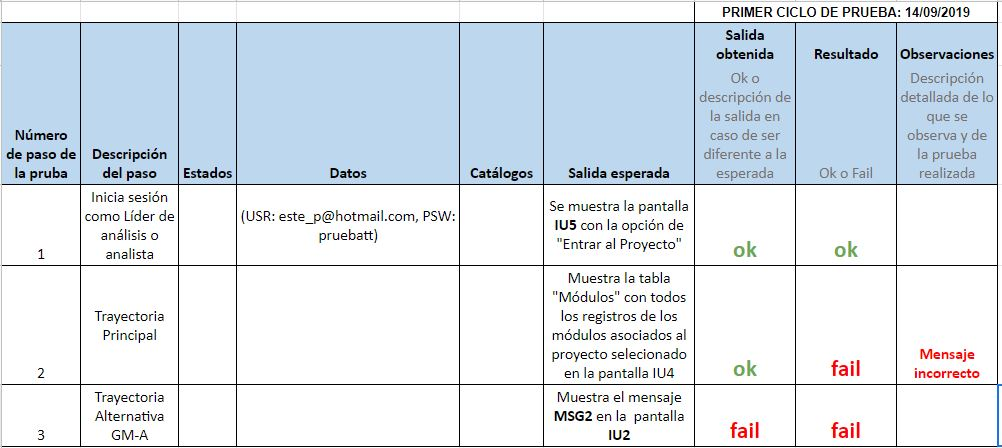
\includegraphics[width=.95\textwidth]{images/pruebas/diseno/tabla}
		\caption{Ejemplo de la estructura de la matriz de pruebas}
		\label{fig:estructura}
	\end{center}
\end{figure}


La ejecución de pruebas se lleva a cabo una vez terminado el desarrollo de cada uno de los sprints estructurados en la metodología.\\

\subsubsection{REPORTE DE PRUEBAS SPRINT 1, 2 y 3 - CICLO 1}

Las pruebas contempladas para el primer ciclo de pruebas abarcan los Casos de Uso del Sprint 1, 2 y 3, Los cuales comprenden las siguientes gestiones:

\begin{itemize}
	\item CU1 Iniciar sesión.
	\item CU2 Gestionar proyectos de Administrador.
	\item CU3 Gestionar Colaboradores.
	\item CU4 Gestionar Proyectos de Colaborador.
\end{itemize}

Se realizaron pruebas dinámicas de sistema, con técnicas de caja negra.\\

Base de prueba:
\begin{itemize}
	\item Casos de Uso
	\item Especificaciónes de requisitos del sistema y software.
	\item Sistema y manual de usuario.
\end{itemize}

Objeto de prueba:
\begin{itemize}
	\item Sistema de software
\end{itemize}

\newpage

Los resultados finales del primer ciclo de prueba arrojaron los siguientes datos:\\

En la Figura \ref{fig:infos1c1} se presenta un informe de los defectos detectados para los sprints 1, 2 y 3. En relación con el tipo de defecto y su severidad, se obtuvieron un total de 13 defectos siendo 1 defecto crítico funcional el más relevante.

\begin{figure}[H]
	\begin{center}
		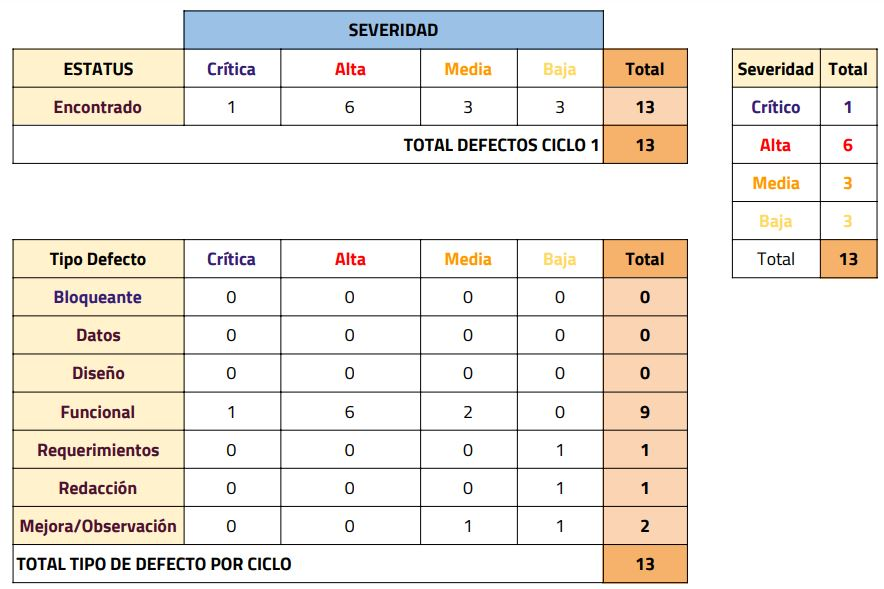
\includegraphics[width=.95\textwidth]{images/pruebas/s1c1}
		\caption{Informe de defectos Sprint 1, 2 y 3 Ciclo 1}
		\label{fig:infos1c1}
	\end{center}
\end{figure}

\newpage

En la gráfica de la Figura \ref{fig:infos1c1-1} se ilustra la representación del comportamiento de los defectos detectados con base en su severidad, esto para los sprints 1, 2 y 3.

\begin{figure}[H]
	\begin{center}
		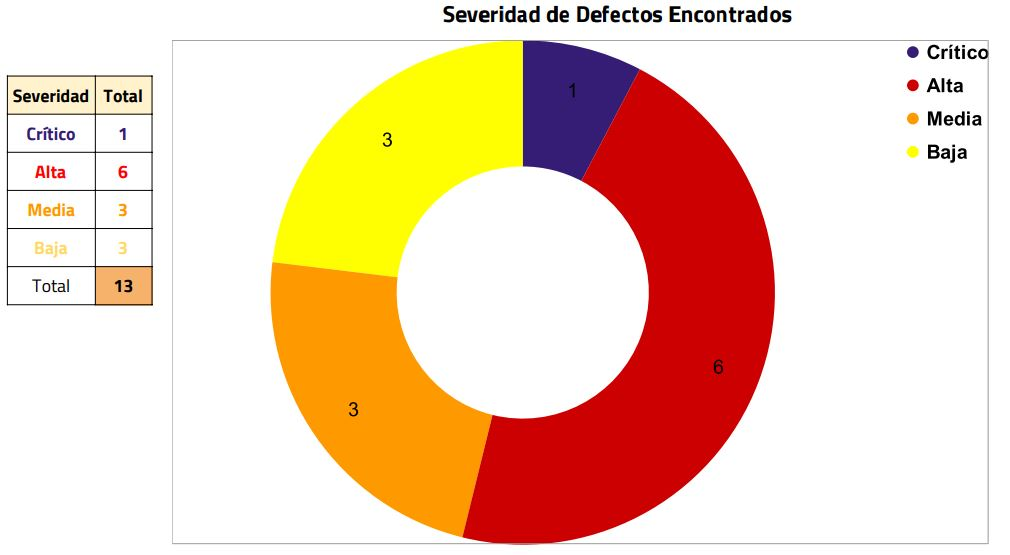
\includegraphics[width=.75\textwidth]{images/pruebas/s1c1-1}
		\caption{Gráfica de defectos por severidad Sprint 1, 2 y 3 Ciclo 1}
		\label{fig:infos1c1-1}
	\end{center}
\end{figure}

En la gráfica de la Figura \ref{fig:infos1c1-2} se ilustra la representación del comportamiento de los defectos detectados con base en su tipo, esto para los sprints 1, 2 y 3.

\begin{figure}[H]
	\begin{center}
		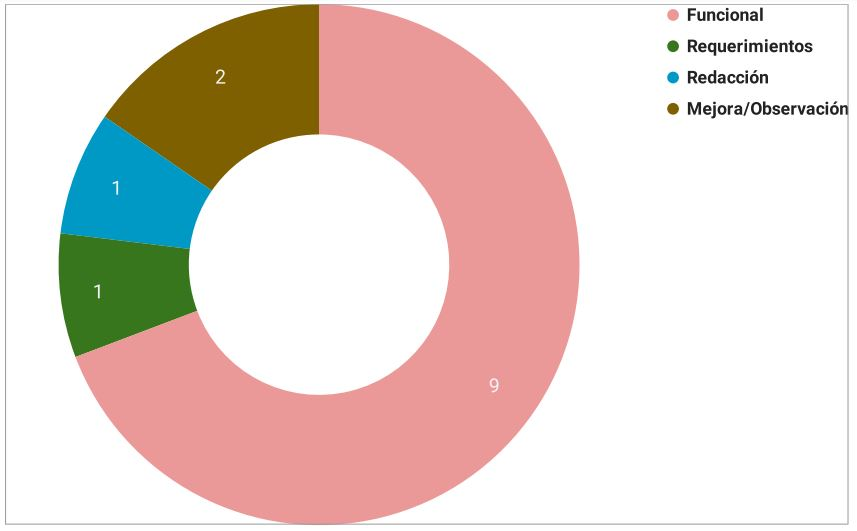
\includegraphics[width=.65\textwidth]{images/pruebas/s1c1-2}
		\caption{Gráfica de defectos por tipo de defecto Sprint 1, 2 y 3 Ciclo 1}
		\label{fig:infos1c1-2}
	\end{center}
\end{figure}

\newpage

En la gráfica de la Figura \ref{fig:infos1c1-3} se ilustra la representación del comportamiento de los defectos detectados con relación en su tipo y severidad, esto para los sprints 1, 2 y 3.

\begin{figure}[H]
	\begin{center}
		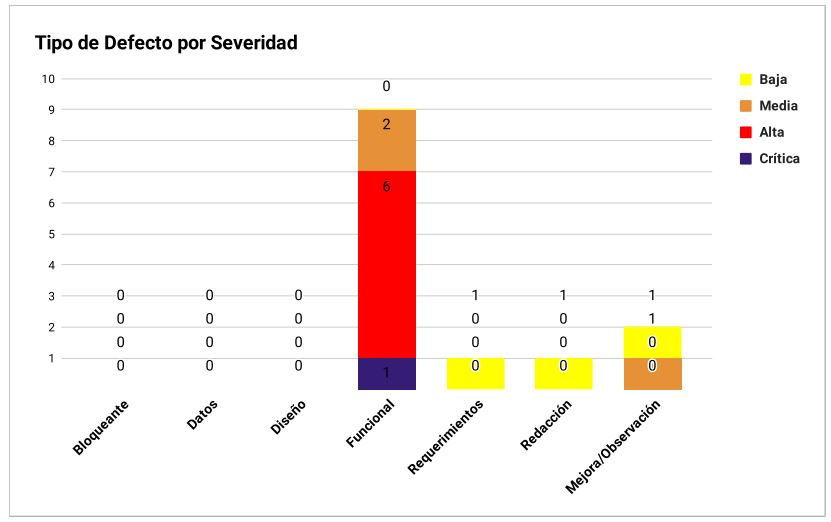
\includegraphics[width=.95\textwidth]{images/pruebas/s1c1-3}
		\caption{Gráfica de tipo de defectos por severidad Sprint 1, 2 y 3 Ciclo 1}
		\label{fig:infos1c1-3}
	\end{center}
\end{figure}

Se corrigieron los defectos encontrados en el primer ciclo.
\newpage

\subsubsection{REPORTE DE PRUEBAS SPRINT 4, 5 y 6 - CICLO 1}
Las pruebas contempladas para el segundo ciclo de pruebas abarcan los Casos de Uso del Sprint 4, 5 y 6, Los cuales comprenden las siguientes gestiones:

\begin{itemize}
	\item CU5 Gestionar Módulos.
	\item CU6 Gestionar Términos del glosario.
	\item CU7 Gestionar Entidades
\end{itemize}

Los resultados finales del primer ciclo de prueba arrojaron los siguientes datos:\\

En la Figura \ref{fig:infos4c2} se presenta un informe de los defectos detectados para los sprints 4, 5 y 6. En relación con el tipo de defecto y su severidad, se obtuvieron un total de 6 defectos siendo 1 defecto crítico bloqueante el más relevante.

\begin{figure}[H]
	\begin{center}
		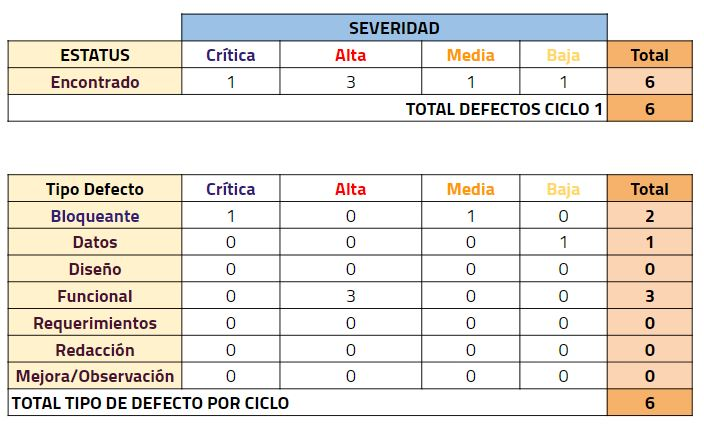
\includegraphics[width=.95\textwidth]{images/pruebas/s4c2}
		\caption{Informe de defectos Sprint 4, 5 y 6  Ciclo 1}
		\label{fig:infos4c2}
	\end{center}
\end{figure}

En la gráfica de la Figura \ref{fig:infos4c2-1} se ilustra la representación del comportamiento de los defectos detectados con base en su severidad, esto para los sprints 4, 5 y 6.

\begin{figure}[H]
	\begin{center}
		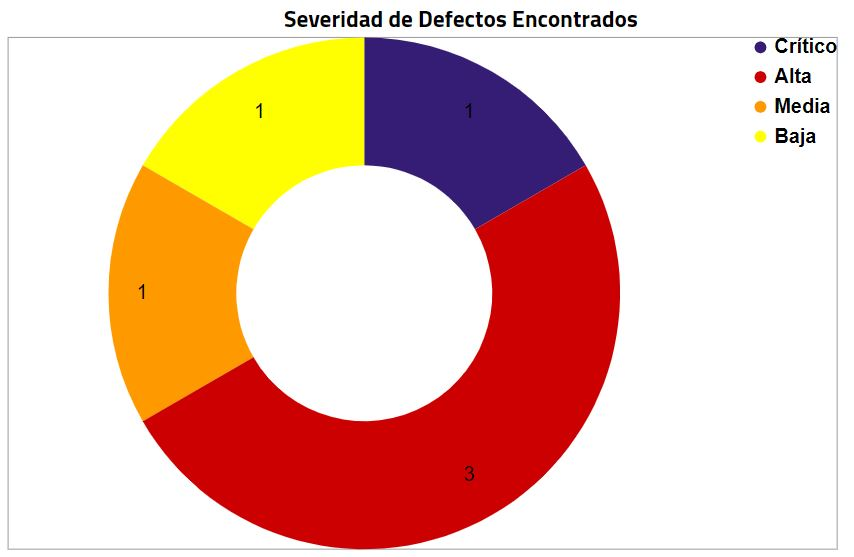
\includegraphics[width=.65\textwidth]{images/pruebas/s4c2-1}
		\caption{Gráfica de defectos por severidad Sprint 4, 5 y 6  Ciclo 1}
		\label{fig:infos4c2-1}
	\end{center}
\end{figure}

En la gráfica de la Figura \ref{fig:infos4c2-2} se ilustra la representación del comportamiento de los defectos detectados con base en su tipo, esto para los sprints 4, 5 y 6.

\begin{figure}[H]
	\begin{center}
		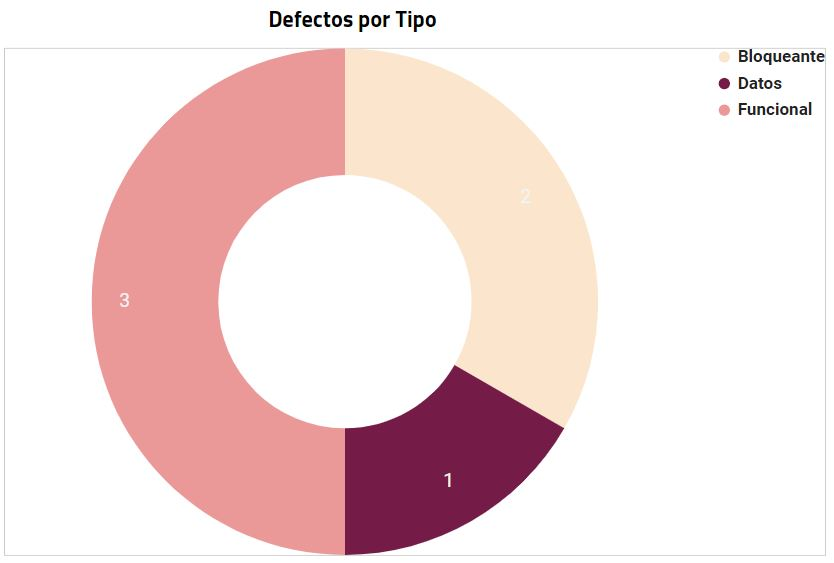
\includegraphics[width=.65\textwidth]{images/pruebas/s4c2-2}
		\caption{Gráfica de defectos por tipo de defecto Sprint 4, 5 y 6  Ciclo 1}
		\label{fig:infos4c2-2}
	\end{center}
\end{figure}

\subsubsection{REPORTE DE PRUEBAS SPRINT 7, 8 y 9 - CICLO 2}

Las pruebas contempladas para el segundo ciclo de pruebas abarcan los Casos de Uso del Sprint 7, 8 y 9, Los cuales comprenden las siguientes gestiones:

\begin{itemize}
	\item CU5 Gestionar Atributos.
	\item CU6 Gestionar Reglas de negocio.
	\item CU7 Gestionar Mensajes.
\end{itemize}

Los resultados finales del segundo ciclo de prueba arrojaron los siguientes datos:\\

En la Figura \ref{fig:infos7c2} se presenta un informe de los defectos detectados para los sprints 7, 8 y 9. En relación con el tipo de defecto y su severidad, se obtuvieron un total de 4 defectos teniendo 2 defectos altos funcionales como más relevantes.

\begin{figure}[H]
	\begin{center}
		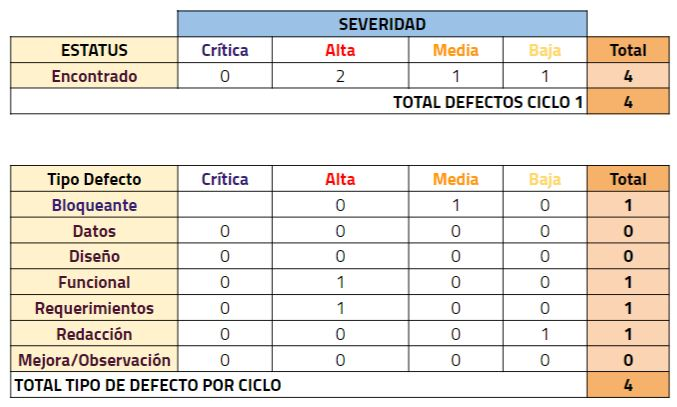
\includegraphics[width=.75\textwidth]{images/pruebas/s7c2}
		\caption{Informe de defectos Sprint 7, 8 y 9  Ciclo 2}
		\label{fig:infos7c2}
	\end{center}
\end{figure}

En la gráfica de la Figura \ref{fig:infos7c2-1} se ilustra la representación del comportamiento de los defectos detectados con base en su severidad, esto para los sprints 7, 8 y 9.

\begin{figure}[H]
	\begin{center}
		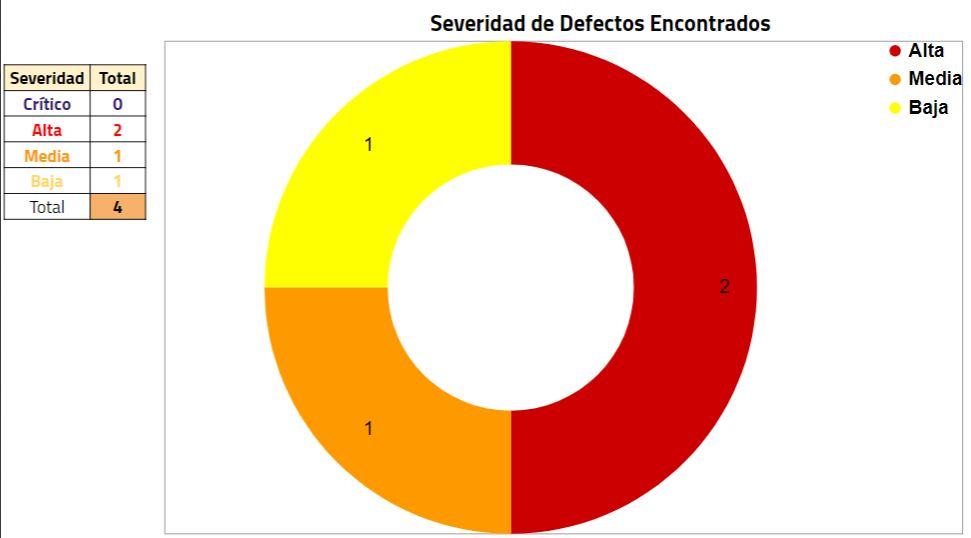
\includegraphics[width=.75\textwidth]{images/pruebas/s7c2-1}
		\caption{Gráfica de defectos por severidad Sprint 7, 8 y 9  Ciclo 2}
		\label{fig:infos7c2-1}
	\end{center}
\end{figure}

En la gráfica de la Figura \ref{fig:infos7c2-2} se ilustra la representación del comportamiento de los defectos detectados con base en su tipo, esto para los sprints 7, 8 y 9.

\begin{figure}[H]
	\begin{center}
		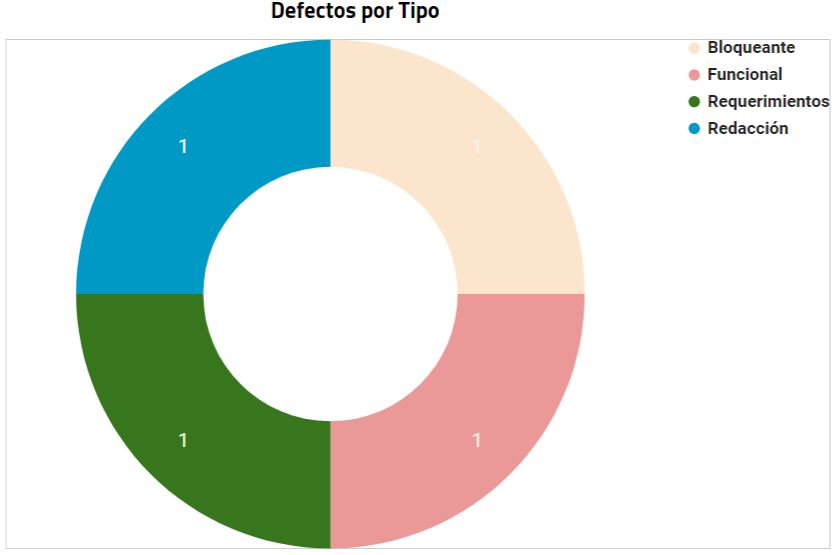
\includegraphics[width=.75\textwidth]{images/pruebas/s7c2-2}
		\caption{Gráfica de defectos por tipo de defecto Sprint 7, 8 y 9  Ciclo 2}
		\label{fig:infos7c2-2}
	\end{center}
\end{figure}

\subsubsection{REPORTE DE PRUEBAS SPRINT 10, 11 y 12 - CICLO 2}

Las pruebas contempladas para el segundo ciclo de pruebas abarcan los Casos de Uso del Sprint 10, 11 y 12, Los cuales comprenden las siguientes gestiones:

\begin{itemize}
	\item CU8 Gestionar Actores.
	\item CU9 Gestionar Pantallas.
	\item CU10 Gestionar Acciones.
\end{itemize}

Los resultados finales del segundo ciclo de prueba arrojaron los siguientes datos:\\

En la Figura \ref{fig:infos10c2} se presenta un informe de los defectos detectados para los sprints 10, 11 y 12. En relación con el tipo de defecto y su severidad, se obtuvieron un total de 5 defectos teniendo 1 defecto funcional crítico como el más relevante.

\begin{figure}[H]
	\begin{center}
		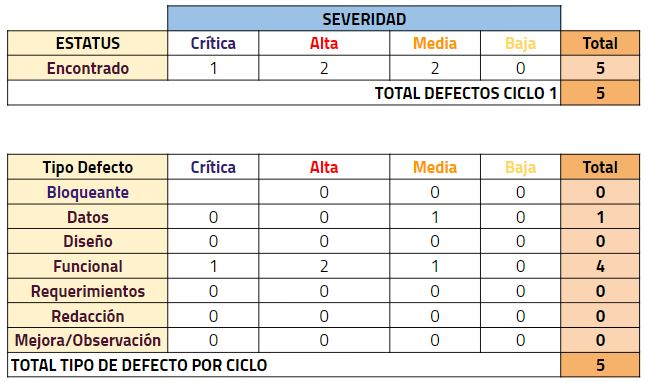
\includegraphics[width=.95\textwidth]{images/pruebas/s10c2}
		\caption{Informe de defectos Sprint 10, 11 y 12  Ciclo 2}
		\label{fig:infos10c2}
	\end{center}
\end{figure}

En la gráfica de la Figura \ref{fig:infos10c2-1} se ilustra la representación del comportamiento de los defectos detectados con base en su severidad, esto para los sprints 7, 8 y 9.

\begin{figure}[H]
	\begin{center}
		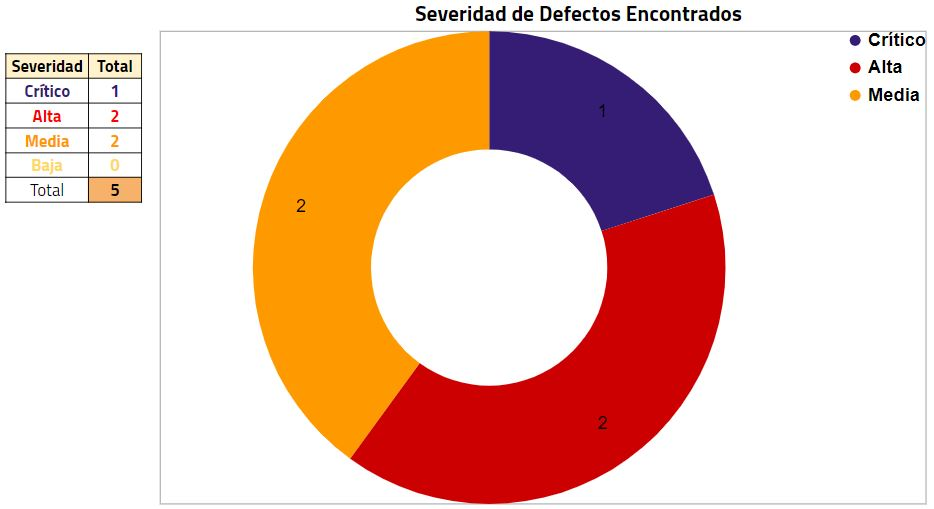
\includegraphics[width=.75\textwidth]{images/pruebas/s10c2-1}
		\caption{Gráfica de defectos por severidad Sprint 10, 11 y 12  Ciclo 2}
		\label{fig:infos10c2-1}
	\end{center}
\end{figure}

En la gráfica de la Figura \ref{fig:infos10c2-2} se ilustra la representación del comportamiento de los defectos detectados con base en su tipo, esto para los sprints 7, 8 y 9.

\begin{figure}[H]
	\begin{center}
		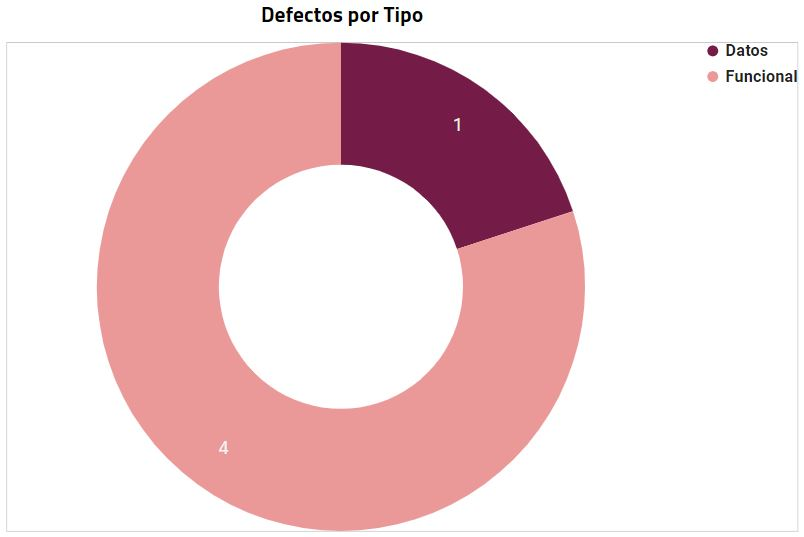
\includegraphics[width=.75\textwidth]{images/pruebas/s10c2-2}
		\caption{Gráfica de defectos por tipo de defecto 10, 11 y 12  Ciclo 2}
		\label{fig:infos10c2-2}
	\end{center}
\end{figure}

\subsubsection{REPORTE DE PRUEBAS SPRINT 13, 14 y 15 - CICLO 3}

Las pruebas contempladas para el tercer ciclo de pruebas abarcan los Casos de Uso del Sprint 13, 14 y 15, Los cuales comprenden las siguientes gestiones:

\begin{itemize}
	\item CU11.1.1 Gestionar Acciones.
	\item CU12.1.1 Gestionar Trayectorias.
	\item CU12.1.1.1 Gestionar Pasos.
\end{itemize}

Los resultados finales del segundo ciclo de prueba arrojaron los siguientes datos:\\

En la Figura \ref{fig:infos13c3} se presenta un informe de los defectos detectados para los sprints 13, 14 y 15. En relación con el tipo de defecto y su severidad, se obtuvieron un total de 3 defectos teniendo 1 defecto funcional alto como el más relevante.

\begin{figure}[H]
	\begin{center}
		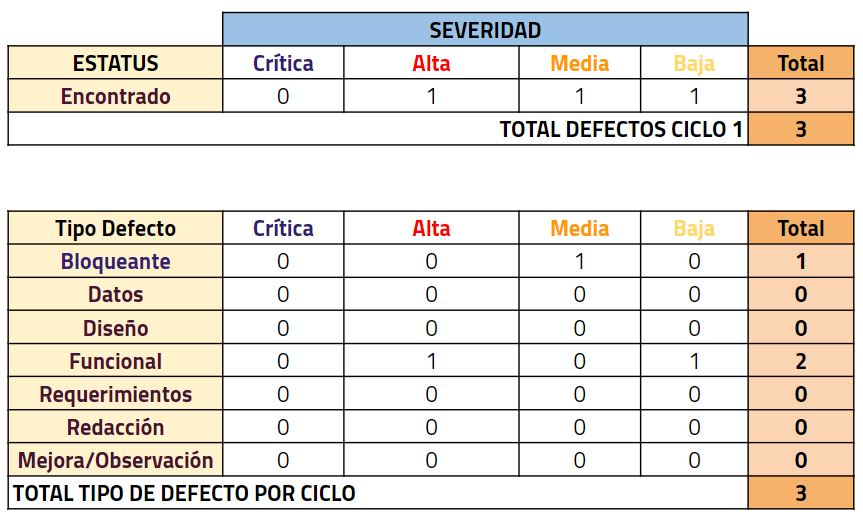
\includegraphics[width=.95\textwidth]{images/pruebas/s13c3}
		\caption{Informe de defectos Sprint 13, 14 y 15  Ciclo 3}
		\label{fig:infos13c3}
	\end{center}
\end{figure}

En la gráfica de la Figura \ref{fig:infos13c3-1} se ilustra la representación del comportamiento de los defectos detectados con base en su severidad, esto para los sprints 13, 14 y 15.

\begin{figure}[H]
	\begin{center}
		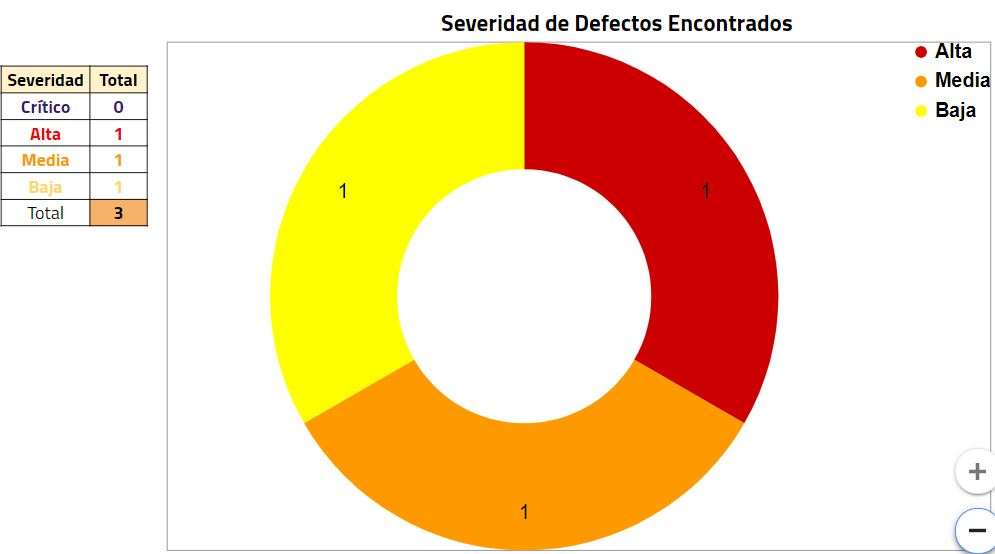
\includegraphics[width=.75\textwidth]{images/pruebas/s13c3-1}
		\caption{Gráfica de defectos por severidad Sprint 13, 14 y 15  Ciclo 3}
		\label{fig:infos13c3-1}
	\end{center}
\end{figure}

En la gráfica de la Figura \ref{fig:infos13c3-2} se ilustra la representación del comportamiento de los defectos detectados con base en su tipo, esto para los sprints 13, 14 y 15.

\begin{figure}[H]
	\begin{center}
		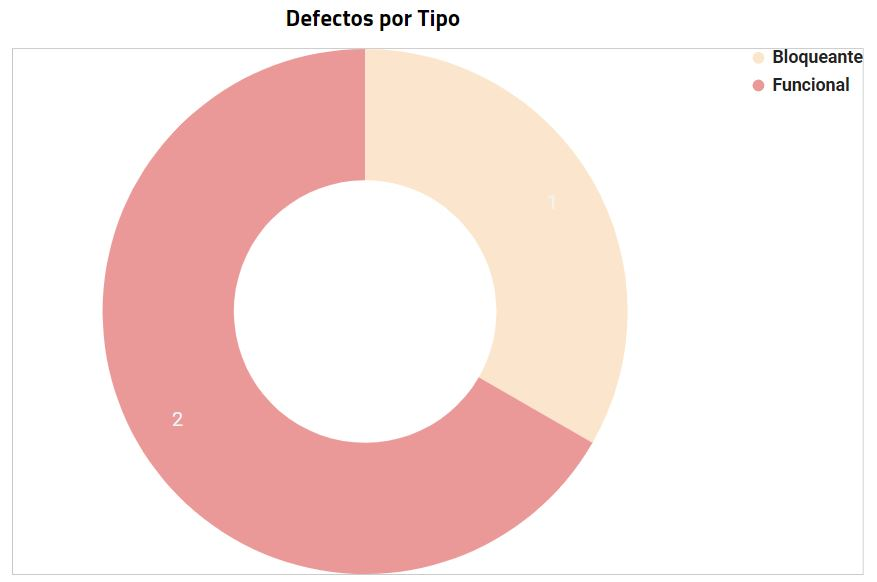
\includegraphics[width=.75\textwidth]{images/pruebas/s13c3-2}
		\caption{Gráfica de defectos por tipo de defecto 13, 14 y 15  Ciclo 3}
		\label{fig:infos13c3-2}
	\end{center}
\end{figure}
\newpage

\section{Pruebas Estáticas}
Como se mencionó al inicio del capítulo, para obtener un producto de calidad no solo se deben realizar pruebas dinámicas, las pruebas estáticas también son necesarias.\\ La herramienta sonarqube nos proporciona un análisis de código exhaustivo, los resultados que nos arrojó se ilustran en la Figura \ref{fig:infoesta}: \\

\begin{figure}[H]
	\begin{center}
		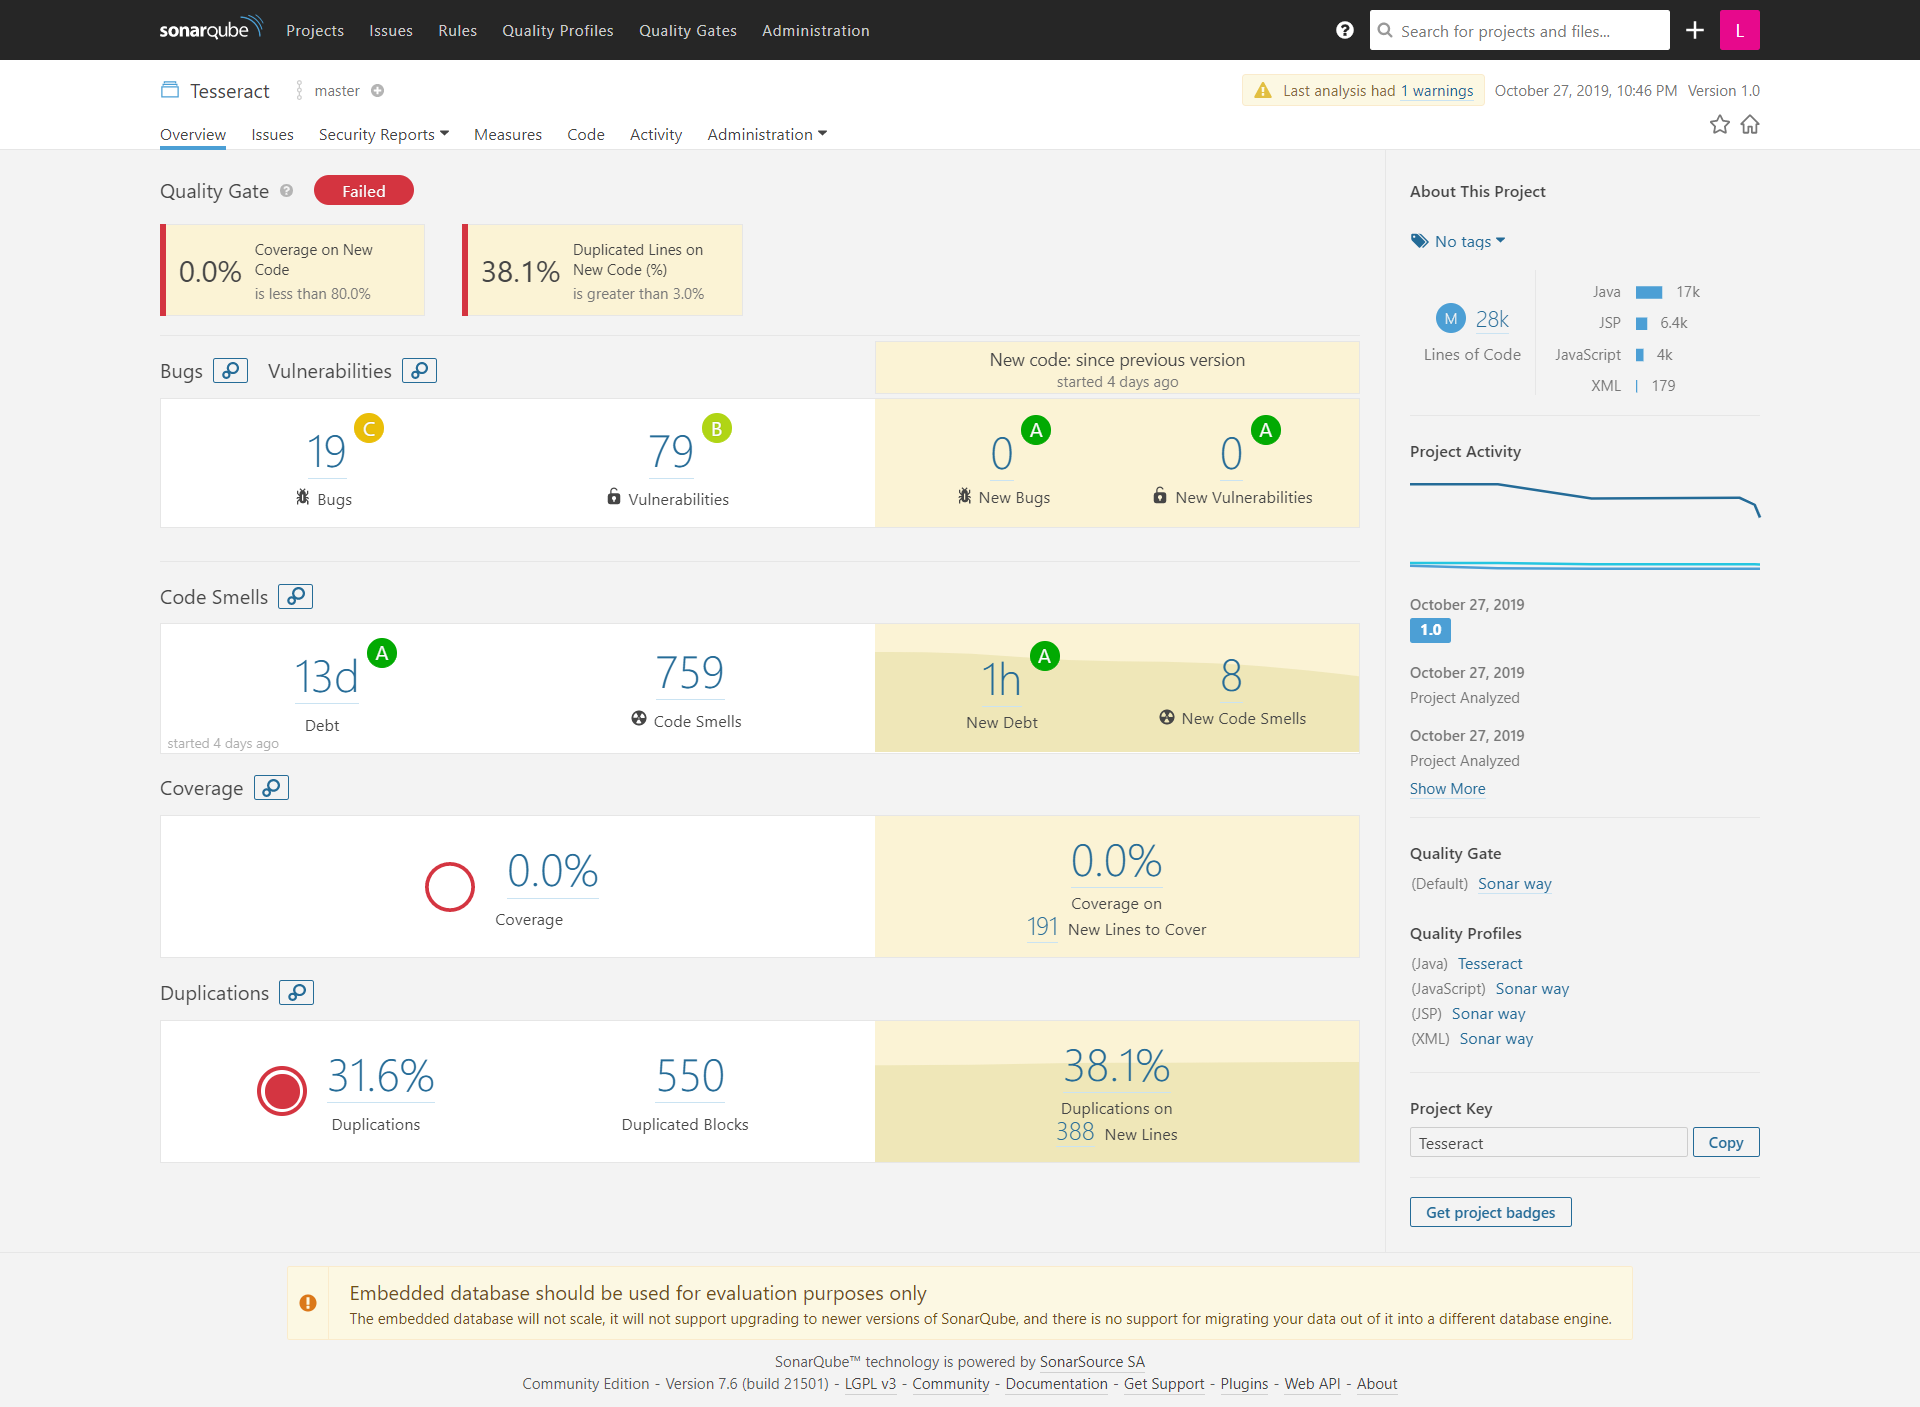
\includegraphics[width=.99\textwidth]{images/pruebas/estaticas/TesseractSonarFirstQualityTest}
		\caption{Reporte de pruebas estáticas SonarQube}
		\label{fig:infoesta}
	\end{center}
\end{figure}
